% This must be in the first 5 lines to tell arXiv to use pdfLaTeX, which is strongly recommended.
\pdfoutput=1
% In particular, the hyperref package requires pdfLaTeX in order to break URLs across lines.

\documentclass[11pt]{article}

% Remove the "review" option to generate the final version.
\usepackage[review]{ACL2023}

% Standard package includes
\usepackage{times}
\usepackage{latexsym}
% For proper rendering and hyphenation of words containing Latin characters (including in bib files)
\usepackage[T1]{fontenc}
% For Vietnamese characters
% \usepackage[T5]{fontenc}
% See https://www.latex-project.org/help/documentation/encguide.pdf for other character sets

% This assumes your files are encoded as UTF8
\usepackage[utf8]{inputenc}
% \usepackage{natbib}
% This is not strictly necessary, and may be commented out.
% However, it will improve the layout of the manuscript,
% and will typically save some space.
\usepackage{microtype}
% This is also not strictly necessary, and may be commented out.
% However, it will improve the aesthetics of text in
% the typewriter font.
\usepackage{inconsolata}
\usepackage[acronym]{glossaries}
\usepackage{graphicx}

\newacronym{llm}{LLM}{large language model}
\newacronym{llm2}{LLM}{large language models}


% If the title and author information does not fit in the area allocated, uncomment the following
%
%\setlength\titlebox{<dim>}
%
% and set <dim> to something 5cm or larger.

\title{Instructions for ACL 2023 Proceedings}

% Author information can be set in various styles:
% For several authors from the same institution:
% \author{Author 1 \and ... \and Author n \\
%         Address line \\ ... \\ Address line}
% if the names do not fit well on one line use
%         Author 1 \\ {\bf Author 2} \\ ... \\ {\bf Author n} \\
% For authors from different institutions:
% \author{Author 1 \\ Address line \\  ... \\ Address line
%         \And  ... \And
%         Author n \\ Address line \\ ... \\ Address line}
% To start a seperate ``row'' of authors use \AND, as in
% \author{Author 1 \\ Address line \\  ... \\ Address line
%         \AND
%         Author 2 \\ Address line \\ ... \\ Address line \And
%         Author 3 \\ Address line \\ ... \\ Address line}

\author{First Author \\
  Affiliation / Address line 1 \\
  Affiliation / Address line 2 \\
  Affiliation / Address line 3 \\
  \texttt{email@domain} \\\And
  Second Author \\
  Affiliation / Address line 1 \\
  Affiliation / Address line 2 \\
  Affiliation / Address line 3 \\
  \texttt{email@domain} \\}

\nolinenumbers
\begin{document}
\maketitle

\section{Introduction}
As technologies continue to advance, the integration of robots into every day life is continuing to increase. As humans rely mostly on speech for communication and instruction, it is essential that robots are also developed to understand and decipher language, executing commands via language effectively and efficiently. 

In this project, we explore the application of reinforcement learning (RL) to train an agent capable of navigating a 2D grid environment and identifying geometric shapes with distinct colors. The agent moves one space at a time across the grid, using RL techniques to learn an optimal policy for efficiently locating and identifying shapes such as green triangles and red squares. We define the task as a partially observable Markov decision process (POMDP), where the agent's observations are limited to the grid space it occupies. Our approach involves implementing Reinforcement Learning to teach the agent to maximize rewards by minimizing the time and steps required to find and correctly identify a shape. The results demonstrate how reinforcement learning can be applied to shape recognition and navigation tasks, with potential applications in robotics, search-and-rescue missions, and autonomous systems. If time permits, we want to further explore what modifications need to be made in order to command a fleet of agents to accomplish tasks in an optimal manner.

\section{Related Work}
Most of the work in this project will be based on the work done by \cite{Chaplot2017}. They utilize a combination of large language models and reinforcement learning to help an agent understand specific instructions to navigate in the game environment of doom. Others utlized the world of minecraft to help agents complete tasks, with less of a focus on instruction and more on generalized learning rather than interpreting language \cite{Oh2017}, \cite{Tessler2020}. Combining the implementation of \cite{Chaplot2017} with the Minigrid environment \cite{MinigridMiniworld23}, \cite{chevalier2018babyai} we can further explore the challenging problem of robotic instruction with large language models. 

\section{Experimental Design}

\begin{figure*}[t]
  \centering
  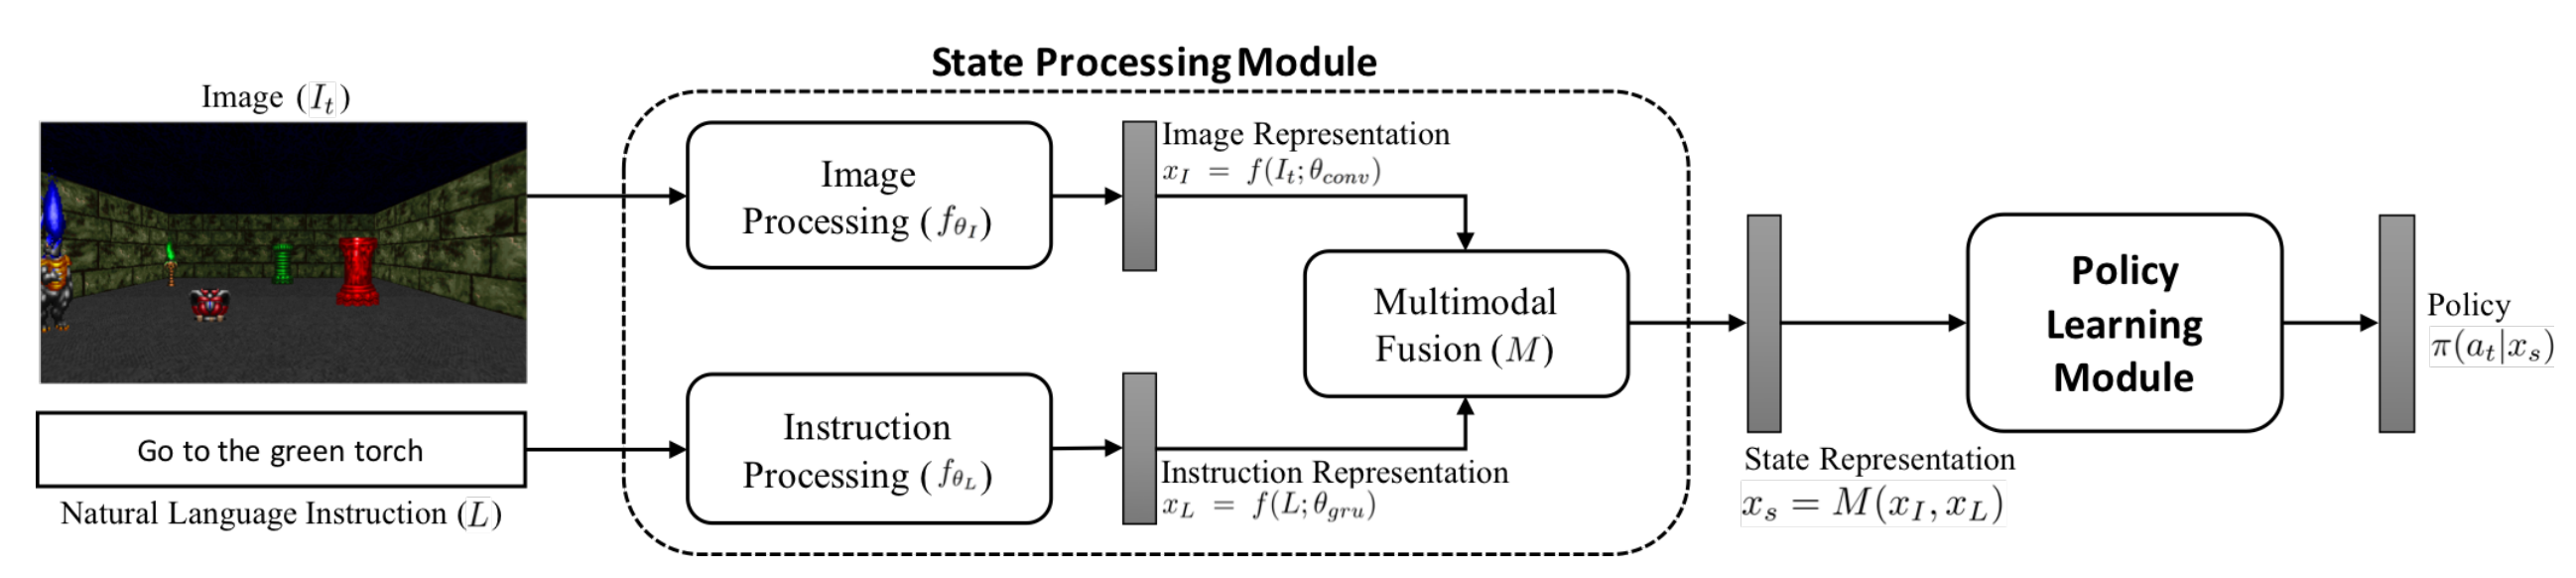
\includegraphics[width=\linewidth]{figs/stateprocessing.png}
  \caption{State processing method as developed by \cite{Chaplot2017}}
  \label{fig:stateprocess}
\end{figure*}

Using a similiar setup as noted in Figure~\ref{fig:stateprocess}, we will use the Minigrid environment in place of DOOM to train our agent to complete specified tasks. 

% Entries for the entire Anthology, followed by custom entries
\bibliography{custom}
\bibliographystyle{plain}


\appendix

\section{Example Appendix}
\label{sec:appendix}

This is a section in the appendix.

\end{document}
